% !TeX spellcheck = fr_FR

% TODO: Replace scan images with clean text where possible

\documentclass[a4paper, 10pt]{report}

\usepackage[french]{babel}
\usepackage[T1]{fontenc}

\usepackage{amsmath, amssymb, amsfonts}

\usepackage{hyperref}
\usepackage{geometry}

\usepackage{xcolor}
\usepackage{graphicx}
\usepackage{subcaption}
\usepackage{tikz}

\usepackage{fancyhdr}
\usepackage{lastpage}

\usepackage{enumitem}

\geometry{
	a4paper,
	left=25mm,
	right=25mm,
	top=35mm,
	bottom=25mm,
	headsep=5mm,
	headheight=20mm,
}

\definecolor{solution}{HTML}{E5E4E2}
\providecommand{\abs}[1]{\lvert#1\rvert}
\providecommand{\norm}[1]{\lVert#1\rVert}
\DeclareMathOperator{\card}{card}

\makeatletter
\renewcommand*\env@matrix[1][*\c@MaxMatrixCols c]{%
	\hskip -\arraycolsep
	\let\@ifnextchar\new@ifnextchar
	\array{#1}}
\makeatother

\begin{document}
	
	\renewcommand{\headrule}{%
		\vspace{-4pt}\hrulefill
		\raisebox{-6.8pt}{\ 
\includegraphics[height=5mm]{../../icon.png}}
		\hrulefill
	}	
	\pagestyle{fancy}
	\fancyhf{}
	
	\fancyhead[L]{\small \slshape Automne 2024}
	\fancyhead[C]{\Large \bfseries Algèbre I - Série 09}
	\fancyhead[R]{\small Buff Mathias}
	\fancyfoot[L]{
		\small Source files available at:
		\href{https://github.com/MathiasBuff/bsc-math}
		{github.com/MathiasBuff/bsc-math}
	}
	\fancyfoot[R]{
		\small Page \thepage
		\hspace{1pt} /
		\pageref*{LastPage}
	}
	

	\noindent
	\textbf{Exercice 1.} (Calcul de déterminant)\\
	En développant par rapport à une ligne ou une colonne, calculer le
	déterminant de la matrice
	\[
		A =
		\begin{pmatrix}
			3 & 5 & -2 & 1\\
			0 & 2 & 3 & 1\\
			1 & 0 & 4 & 0\\
			-2 & 1 & 1 & 1\\
		\end{pmatrix}
	\]
	
	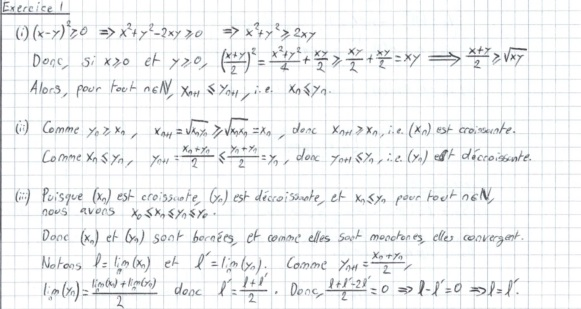
\includegraphics{ex01.jpg}
	
	\vspace{5mm}
	\noindent
	\textbf{Exercice 2.}(Méthode de Gauss)\\
	En utilisant l'élimination de Gauss, calculer le déterminant et
	l'inverse des matrices
	\[
		A =
		\begin{pmatrix}
			1 & 2 & 3\\
			0 & 0 & -1\\
			-2 & 0 & -8\\
		\end{pmatrix}
		\quad \text{et} \quad
		B =
		\begin{pmatrix}
			1 & 1 & 0 & 0\\
			1 & 1 & 1 & 0\\
			0 & 1 & 1 & 1\\
			0 & 0 & 1 & 1\\
		\end{pmatrix}
	\]
	\textbf{Indication :} Considérer la matrice augmentée par une matrice
	identité à droite.
	
	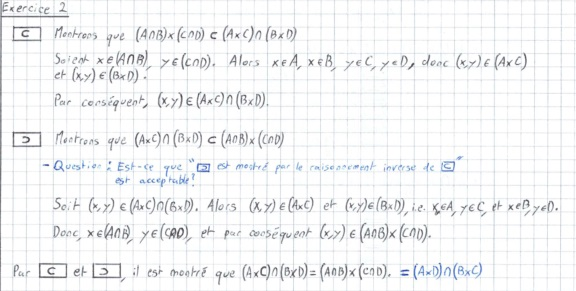
\includegraphics{ex02.jpg}
	
	\newpage
	
	\fancyhf{}
	\renewcommand{\headrule}
	{\rule{\textwidth}{0pt}}
	\fancyfoot[R]{
		\small Page \thepage
		\hspace{1pt} /
		\pageref*{LastPage}
	}
	
	\noindent
	\textbf{Exercice 3.} (Comatrice et cofacteurs)\\
	Calculer l'inverse des matrices suivantes en passant par les cofacteurs
	\[
	A =
	\begin{pmatrix}
		1 & 2 & 3\\
		0 & 0 & -1\\
		-2 & 0 & -8\\
	\end{pmatrix}
	,\quad
	B =
	\begin{pmatrix}
		1 & x & z\\
		0 & 1 & y\\
		0 & 0 & 1\\
	\end{pmatrix}
	\quad \text{et} \quad
	C =
	\begin{pmatrix}
		0 & 1 & 0 & 0\\
		0 & 0 & 1 & 0\\
		0 & 0 & 0 & 1\\
		1 & 0 & 0 & 0\\
	\end{pmatrix}
	\]
	
	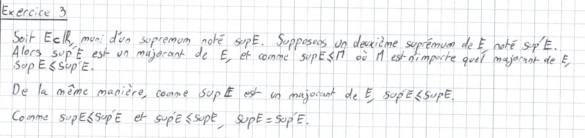
\includegraphics{ex03.jpg}
	
	\newpage
	
	\noindent
	\textbf{Exercice 4.}(Interprétation géométrique du déterminant)
	\begin{enumerate}[label = (\alph*)]
		\item Montrer que l'aire du parallélogramme engendré par deux
		vecteurs $v, w \in \mathbb{R}^2$ (\textit{i.e.} le parallélogramme
		dont les sommets sont $0, v, v+w, w$) est égale au déterminant de
		la matrice $2 \times 2$ dont les lignes sont données par les
		vecteurs $v, w$.
		\begin{figure}[h]\centering
		\begin{subfigure}[c]{0.4\textwidth}
		\begin{tikzpicture}
			\draw[->] (-1.5,0) -- (3,0) node[right]{};
			\draw[->] (0,-1.5) -- (0,3) node[above]{};
			
			\fill [fill=blue!20, draw=blue, thick]
				(0,0)		node [circle, fill=blue, inner sep=1.5pt] {}
			-- 	(1.5,2)		node [circle, fill=blue, inner sep=1.5pt] {}
			-- 	(3.5,2.5)	node [circle, fill=blue, inner sep=1.5pt] {}
			-- 	(2,0.5)		node [circle, fill=blue, inner sep=1.5pt] {}
			--	(0,0);
			
			\node at (1,2.3) {$w = (c, d)$};
			\node at (3,0.5) {$v = (a, b)$};
		\end{tikzpicture}\end{subfigure}
		\begin{subfigure}[c]{0.2\textwidth}
		Aire $\overset{?}{=}\det \begin{pmatrix}a & b\\ c & d\\\end{pmatrix}$
		\end{subfigure}
		\end{figure}
		
		\textit{Indice : Étudiez comment la figure / l'aire évolue quand
		on remplace $w$ par $w - \lambda v$.}
		
		\colorbox{solution}
		{\begin{minipage}{0.9\textwidth}
			\begin{minipage}{0.35\textwidth}
				\begin{tikzpicture}
					\fill [fill=orange!20, draw=orange, thick]
					(0,0)			node  {}
					-- 	(1.5,2)		node  {}
					-- 	(0,2)		node  {}
					--	(0,0);
					
					\fill [fill=red!20, draw=red, thick]
					(0,0)			node  {}
					-- 	(2,0)		node  {}
					-- 	(2,0.5)		node  {}
					--	(0,0);
					
					\fill [fill=teal!20, draw=teal, thick]
					(1.5,2)			node  {}
					-- 	(2,2)		node  {}
					-- 	(2,0.5)		node  {}
					--	(1.5,2);
					
					\fill [fill=blue!20, draw=blue, thick]
					(0,0)			node [circle, fill=blue, inner sep=1.5pt] {}
					-- 	(1.5,2)		node [circle, fill=blue, inner sep=1.5pt] {}
					-- 	(2,0.5)		node [circle, fill=blue, inner sep=1.5pt] {}
					--	(0,0);
					
					\draw[->] (-1.5,0) -- (3,0) node[right]{};
					\draw[->] (0,-1.5) -- (0,3) node[above]{};
					
					\node at (1.5,2.3) {$w$};
					\node at (2.3,0.5) {$v$};
					\node at (2,-0.3) {$e$};
					\node at (-0.3,2) {$f$};
					\node at (2.15,2.15) {$g$};
				\end{tikzpicture}
			\end{minipage}
			\begin{minipage}{0.5\textwidth}
				Observons que l'aire du triangle $0vw$ est égale à la moitié
				de celle du parallélogramme. Soient les points 
				$e = (a,0), f = (0,d), g = (a,d)$. Alors
				\[\begin{aligned}
					{\color{blue}A(0vw)} &= A(0egf) - {\color{red}A(0ev)}
						- {\color{orange}A(0wf)} - {\color{teal}A(vgw)}\\
					&= ad - {\color{red}\frac{ab}{2}}
						- {\color{orange}\frac{cd}{2}}
						- {\color{teal}\frac{(d-b)(a-c)}{2}}\\
					&= ad - {\color{red}\frac{ab}{2}}
						- {\color{orange}\frac{cd}{2}}
						- {\color{teal}\frac{ad}{2} + \frac{ab}{2}
							+ \frac{cd}{2} - \frac{bc}{2}}\\
					&= \frac{ad}{2} - \frac{bc}{2}\\
					&= {\color{blue}\frac{ad - bc}{2}}
				\end{aligned}\]
			\end{minipage}\\
		
			On conclut que l'aire du parallélogramme est égale à
			$2 \cdot \frac{ad - bc}{2} = ad - bc$.
		\end{minipage}}
		
		\item En déduire que
		\[
			\det \begin{pmatrix}a & b\\ c & d\\\end{pmatrix} = 0 \iff
			\mathrm{rank}\begin{pmatrix}a & b\\ c & d\\\end{pmatrix} < 2
		\]
		Donner une condition géométrique qui est également équivalente à
		ces deux conditions.
		
		\colorbox{solution}
		{\begin{minipage}{0.9\textwidth}
			Si $\det \left(\begin{smallmatrix}a & b\\
				c & d\\\end{smallmatrix}\right) = 0$, alors l'aire du
			parallélogramme correspondant est nulle. On en déduit que
			l'image formée par $\vec{v}$ et $\vec{w}$ est une ligne ou
			un point, ainsi la dimension de cette image est inférieure
			à la dimension du plan. Comme le rang d'une matrice est égal
			au rang de sa transposée, on conclut que
			\[
				\det \begin{pmatrix}a & b\\ c & d\\\end{pmatrix} = 0 \iff
				\mathrm{rank}\begin{pmatrix}a & c\\ b & d\\\end{pmatrix} =
				\mathrm{rank}\begin{pmatrix}a & b\\ c & d\\\end{pmatrix} < 2
			\]
			On observe qu'une telle image est formée si $\vec{v}$ et 
			$\vec{w}$ sont colinéaires.
		\end{minipage}}
		
		\item Comment pourrait-on généraliser les énoncés (a) et (b) en
		dimension supérieure ?
		
		\colorbox{solution}
		{\begin{minipage}{0.9\textwidth}
			Observons que l'aire du parallélogramme vaut 1 dans
			la base formée par les vecteurs $\vec{v}$ et $\vec{w}$.
			Alors le déterminant représente le facteur à appliquer pour
			convertir une aire dans cette base à une aire dans la base
			canonique.\\
			Par analogie, pour un espace de dimension $n$, le déterminant
			d'une matrice carrée de même dimension est égal au $n$-volume
			unitaire de la base formée par les lignes de cette matrice,
			exprimé dans la base canonique de $\mathbb{R}^n$. S'il est
			nul, alors l'espace formé est de dimension inférieure.
		\end{minipage}}
	\end{enumerate}
	
	\newpage
	
	\noindent
	\textbf{Exercice 5.}(Déterminant de matrice à paramètre)\\
	Considérons la matrice
	\[
	\begin{pmatrix}
		1 & 1 & m\\
		1 & m & 1\\
		m & 1 & 1\\
	\end{pmatrix}
	\]
	\begin{enumerate}[label = (\alph*)]
		\item En utilisant la méthode du pivot, déterminer le rang de $C$.
		Cette valeur dépend de $m \in \mathbb{R}$.
		\item Calculer le déterminant de $C$. La valeur obtenue permet-elle
		de trouver la réponse à la question (a) ?
	\end{enumerate}
	
	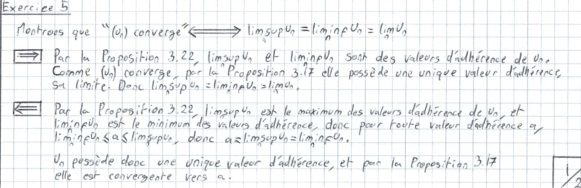
\includegraphics{ex05.jpg}
	
	\vspace{5mm}
	\noindent
	\textbf{Exercice 6.}(Déterminant de matrices particulières)\\
	Calculer le déterminant de la matrice
	\[
	\begin{pmatrix}
		1 & 2 & 3\\
		0 & 4 & 5\\
		0 & 0 & 6\\
	\end{pmatrix}
	\begin{pmatrix}
		1 & 0 & 0\\
		\tfrac{1}{2} & \tfrac{1}{3} & 0\\
		\tfrac{1}{4} & \tfrac{1}{5} & \tfrac{1}{6}\\
	\end{pmatrix}
	\]
	
	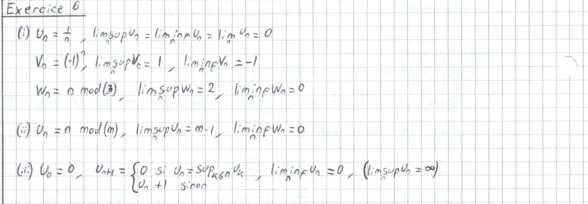
\includegraphics{ex06.jpg}
	
	
%	
%	\colorbox{solution}
%	{
%		\begin{minipage}{0.9\textwidth}
%			s
%		\end{minipage}
%	}
%	
%	\colorbox{solution}
%	{
%		\begin{minipage}{0.9\textwidth}
%			\begin{enumerate}[label=(\alph*)]
%				\item a
%			\end{enumerate}
%		\end{minipage}
%	}
	
\end{document}
